\documentclass{article}

% Same template as projects/monitoramento/manuscript/arrecadacao_forecast_v1 (NeurIPS 2025 style, preprint option).
% Target: AAA congress. Drop the preprint option for an anonymised submission.
% Every number comes from numeros.tex; every figure and table comes from figures/ and tables/,
% all generated by projects/macro/notebooks/articles/icms_declarado_autuado.ipynb (L5). Nothing is typed by hand.
\usepackage[preprint]{neurips_2025}

\usepackage[utf8]{inputenc}
\usepackage[T1]{fontenc}
\usepackage{hyperref}
\usepackage{url}
\usepackage{booktabs}
\usepackage{amsfonts}
\usepackage{amsmath}
\usepackage{amssymb}
% Aliases so inequality signs stay valid if the source is edited as Markdown.
\newcommand{\lt}{<}\newcommand{\gt}{>}
\usepackage{graphicx}
\usepackage{float}
\usepackage[font=normalsize,labelfont=bf,labelsep=period]{caption}
\captionsetup{font={normalsize},labelfont={bf}}
\usepackage{microtype}
\usepackage{xcolor}

% generated by projects/macro/notebooks/articles/icms_declarado_autuado.ipynb; do not edit by hand
% snapshot 2025-12; panel 2016-2025; payments through 31 December 2025; seed 2026
% database: cemepi.duckdb (39812870144 bytes, mtime 1790177521); aggregates only
\newcommand{\cdaAssessedNineteen}{124,498}  % tab_annual_series_origin
\newcommand{\cdaAssessedTwenty}{67,224}  % tab_annual_series_origin
\newcommand{\cnaeAssessedWeightMax}{96.5}  % tab_cnae_division_origin
\newcommand{\cnaeAssessedWeightMin}{0.0}  % tab_cnae_division_origin
\newcommand{\cnaeNDivShown}{72}  % tab_cnae_division_origin
\newcommand{\cnaeNDivSuppressed}{15}  % tab_cnae_division_origin
\newcommand{\cnaePctStockNoCnae}{0.1}  % tab_cnae_division_origin
\newcommand{\cnaeSecondDivision}{47}  % tab_cnae_division_origin
\newcommand{\cnaeSecondDivisionAssessedWeight}{72.5}  % tab_cnae_division_origin
\newcommand{\cnaeSecondDivisionName}{retail trade}  % tab_cnae_division_origin (English name, IBGE CNAE 2.0)
\newcommand{\cnaeSecondDivisionPctStock}{11.8}  % tab_cnae_division_origin
\newcommand{\cnaeSpearman}{-0.51}  % tab_cnae_division_origin
\newcommand{\cnaeTenPctStock}{73.3}  % tab_ms_cnae_top10
\newcommand{\cnaeTopDivision}{46}  % tab_cnae_division_origin
\newcommand{\cnaeTopDivisionAssessedWeight}{85.6}  % tab_cnae_division_origin
\newcommand{\cnaeTopDivisionName}{wholesale trade, except motor vehicles and motorcycles}  % tab_cnae_division_origin (English name, IBGE CNAE 2.0)
\newcommand{\cnaeTopDivisionPctStock}{27.3}  % tab_cnae_division_origin
\newcommand{\cnaeTopFivePctStock}{55.4}  % tab_cnae_division_origin
\newcommand{\firmCovCdaDec}{100.0}  % tab_firm_coverage
\newcommand{\firmCovCdaPanel}{99.9}  % tab_firm_coverage
\newcommand{\firmCovStockDec}{99.9}  % tab_firm_coverage
\newcommand{\firmNCdaPanel}{4,934,322}  % tab_firm_coverage
\newcommand{\firmNCnpjDec}{216,006}  % tab_firm_coverage
\newcommand{\giniDebtorAssessed}{0.896}  % tab_concentration
\newcommand{\giniDebtorDeclared}{0.944}  % tab_concentration
\newcommand{\kFiftyDebtorAssessed}{302}  % tab_concentration
\newcommand{\kFiftyDebtorDeclared}{982}  % tab_concentration
\newcommand{\kFiftyDebtorVat}{550}  % tab_concentration
\newcommand{\kmBestKEuclid}{4}  % tab_kmeans_selection
\newcommand{\kmBestKGower}{4}  % tab_kmeans_selection
\newcommand{\kmCohortAssessedActive}{27,237}  % tab_km_status_origin
\newcommand{\kmCohortAssessedClosed}{8,414}  % tab_km_status_origin
\newcommand{\kmCohortAssessedUnfit}{8,170}  % tab_km_status_origin
\newcommand{\kmCohortDeclaredActive}{2,763,798}  % tab_km_status_origin
\newcommand{\kmCohortDeclaredClosed}{456,680}  % tab_km_status_origin
\newcommand{\kmCohortDeclaredUnfit}{275,792}  % tab_km_status_origin
\newcommand{\kmCohortNAssessed}{44,110}  % tab_km_status_origin
\newcommand{\kmCohortNDeclared}{3,510,539}  % tab_km_status_origin
\newcommand{\kmGFourPctCda}{3.3}  % tab_kmeans_k4_profiles
\newcommand{\kmGFourPctValue}{5.4}  % tab_kmeans_k4_profiles
\newcommand{\kmGOnePctCda}{70.7}  % tab_kmeans_k4_profiles
\newcommand{\kmGOnePctValue}{79.7}  % tab_kmeans_k4_profiles
\newcommand{\kmGThreePctCda}{6.4}  % tab_kmeans_k4_profiles
\newcommand{\kmGThreePctValue}{6.1}  % tab_kmeans_k4_profiles
\newcommand{\kmGTwoPctCda}{19.6}  % tab_kmeans_k4_profiles
\newcommand{\kmGTwoPctValue}{8.8}  % tab_kmeans_k4_profiles
\newcommand{\kmMinValueMn}{1.59}  % top 1% legal entities Dec 2025
\newcommand{\kmN}{23,222}  % top 1% legal entities Dec 2025
\newcommand{\kmNoOriginAri}{0.203}  % tab_kmeans_without_origin
\newcommand{\kmPaidFiveYrAssessedActive}{35.1}  % tab_km_status_origin
\newcommand{\kmPaidFiveYrAssessedClosed}{22.6}  % tab_km_status_origin
\newcommand{\kmPaidFiveYrAssessedUnfit}{6.8}  % tab_km_status_origin
\newcommand{\kmPaidFiveYrDeclaredActive}{36.5}  % tab_km_status_origin
\newcommand{\kmPaidFiveYrDeclaredClosed}{27.5}  % tab_km_status_origin
\newcommand{\kmPaidFiveYrDeclaredUnfit}{10.3}  % tab_km_status_origin
\newcommand{\kmPaidOneYrAssessedActive}{18.9}  % tab_km_status_origin
\newcommand{\kmPaidOneYrAssessedClosed}{11.4}  % tab_km_status_origin
\newcommand{\kmPaidOneYrAssessedUnfit}{2.9}  % tab_km_status_origin
\newcommand{\kmPaidOneYrDeclaredActive}{30.2}  % tab_km_status_origin
\newcommand{\kmPaidOneYrDeclaredClosed}{22.7}  % tab_km_status_origin
\newcommand{\kmPaidOneYrDeclaredUnfit}{8.6}  % tab_km_status_origin
\newcommand{\kmPctPaid}{12.5}  % top 1% legal entities Dec 2025
\newcommand{\kmPurityBase}{78.7}  % tab_kmeans_without_origin
\newcommand{\kmPurityWith}{98.3}  % tab_kmeans_without_origin
\newcommand{\kmPurityWithout}{78.7}  % tab_kmeans_without_origin
\newcommand{\kmSilEuclid}{0.676}  % tab_kmeans_selection k=4
\newcommand{\kmSilGower}{0.661}  % tab_kmeans_selection k=4
\newcommand{\kmSumBn}{324.6}  % top 1% legal entities Dec 2025
\newcommand{\kwRateH}{14,752}  % tab_kruskal_types
\newcommand{\meanValueAssessed}{5,322,754}  % tab_profile_type
\newcommand{\meanValueDeclared}{51,643}  % tab_profile_type
\newcommand{\medianAgeAssessed}{9.26}  % tab_profile_type
\newcommand{\medianAgeDeclared}{4.61}  % tab_profile_type
\newcommand{\medianValueAssessed}{596,311}  % tab_profile_type
\newcommand{\medianValueDeclared}{7,334}  % tab_profile_type
\newcommand{\nCdaAssessed}{59,536}  % tab_bases_dec2025
\newcommand{\nCdaDeclared}{2,254,464}  % tab_bases_dec2025
\newcommand{\nCdaDeclaredMn}{2.25}  % tab_bases_dec2025
\newcommand{\nCdaVat}{2,323,367}  % tab_bases_dec2025
\newcommand{\paidAssessedNineteen}{0.70}  % tab_annual_series_origin
\newcommand{\paidAssessedTwentyFour}{1.18}  % tab_annual_series_origin
\newcommand{\pcaOnePct}{47.1}  % tab_kmeans_pca
\newcommand{\pctAnyPaymentAssessed}{14.4}  % tab_profile_type
\newcommand{\pctAnyPaymentDeclared}{25.9}  % tab_profile_type
\newcommand{\pctCdaAssessed}{2.6}  % tab_bases_dec2025
\newcommand{\pctCdaFiledAssessed}{88.4}  % tab_profile_type
\newcommand{\pctCdaFiledDeclared}{69.7}  % tab_profile_type
\newcommand{\pctCdaPj}{100.00}  % tab_bases_dec2025
\newcommand{\pctStockAssessed}{72.9}  % tab_bases_dec2025
\newcommand{\pctStockFiledAssessed}{91.5}  % tab_profile_type
\newcommand{\pctStockFiledDeclared}{94.2}  % tab_profile_type
\newcommand{\pctStockPj}{99.52}  % tab_bases_dec2025
\newcommand{\qualDecTwentyFourCdas}{1,272,207}  % tab_debito_quality 2024-12 cdas
\newcommand{\qualDecTwentyFourRef}{2,148,025}  % tab_debito_quality 2024-12 ref_median7
\newcommand{\qualDuplicatedSnapshots}{2016-05, 2016-07, 2017-04, 2017-06, 2017-10, 2017-11, 2018-02, 2018-10, 2019-02, 2019-12, 2020-01, 2020-04, 2020-05, 2020-06, 2021-07, 2021-08, 2021-09, 2021-10, 2021-11, 2022-01, 2022-02, 2022-03, 2024-04, 2024-08, 2024-09, 2024-10, 2024-11, 2025-06, 2025-07, 2025-11}  % tab_debito_quality
\newcommand{\qualMissingSnapshots}{2018-12, 2020-10, 2020-11, 2020-12}  % tab_debito_quality
\newcommand{\qualPartialSnapshots}{2018-11, 2021-04, 2021-05, 2021-06, 2023-02, 2023-03, 2023-12, 2024-03, 2024-05, 2024-12}  % tab_debito_quality
\newcommand{\rBisAge}{0.392}  % tab_mannwhitney_origin |r| origin
\newcommand{\rBisRate}{0.125}  % tab_mannwhitney_origin |r| origin
\newcommand{\rBisTypeAge}{0.398}  % tab_mannwhitney_origin |r| raw types
\newcommand{\rBisTypeRate}{0.127}  % tab_mannwhitney_origin |r| raw types
\newcommand{\rBisTypeValue}{0.895}  % tab_mannwhitney_origin |r| raw types
\newcommand{\rBisValue}{0.891}  % tab_mannwhitney_origin |r| origin
\newcommand{\rateMaxAssessed}{0.39}  % tab_annual_series_origin
\newcommand{\rateMaxDeclared}{1.59}  % tab_annual_series_origin
\newcommand{\rateMaxYearAssessed}{2024}  % tab_annual_series_origin
\newcommand{\rateMaxYearDeclared}{2024}  % tab_annual_series_origin
\newcommand{\rateMinAssessed}{0.03}  % tab_annual_series_origin
\newcommand{\rateMinDeclared}{0.77}  % tab_annual_series_origin
\newcommand{\rateMinYearAssessed}{2018}  % tab_annual_series_origin
\newcommand{\rateMinYearDeclared}{2019}  % tab_annual_series_origin
\newcommand{\rateTwentyFiveAssessed}{0.21}  % tab_annual_series_origin 2025
\newcommand{\rateTwentyFiveDeclared}{1.51}  % tab_annual_series_origin 2025
\newcommand{\restOnePctCdaAssessed}{1.8}  % tab_top_composition
\newcommand{\restOnePctValueAssessed}{16.6}  % tab_top_composition
\newcommand{\stAnyPayAssessedActive}{30.8}  % tab_status_recovery
\newcommand{\stAnyPayAssessedClosed}{8.0}  % tab_status_recovery
\newcommand{\stAnyPayAssessedSuspended}{14.0}  % tab_status_recovery
\newcommand{\stAnyPayAssessedUnfit}{5.5}  % tab_status_recovery
\newcommand{\stAnyPayDeclaredActive}{30.4}  % tab_status_recovery
\newcommand{\stAnyPayDeclaredClosed}{16.9}  % tab_status_recovery
\newcommand{\stAnyPayDeclaredSuspended}{13.9}  % tab_status_recovery
\newcommand{\stAnyPayDeclaredUnfit}{7.0}  % tab_status_recovery
\newcommand{\stCnpjAssessedActive}{15,640}  % tab_status_recovery
\newcommand{\stCnpjAssessedClosed}{7,625}  % tab_status_recovery
\newcommand{\stCnpjAssessedSuspended}{275}  % tab_status_recovery
\newcommand{\stCnpjAssessedUnfit}{9,243}  % tab_status_recovery
\newcommand{\stCnpjDeclaredActive}{142,869}  % tab_status_recovery
\newcommand{\stCnpjDeclaredClosed}{29,882}  % tab_status_recovery
\newcommand{\stCnpjDeclaredSuspended}{806}  % tab_status_recovery
\newcommand{\stCnpjDeclaredUnfit}{20,994}  % tab_status_recovery
\newcommand{\stPctStockAssessedActive}{52.9}  % tab_status_recovery
\newcommand{\stPctStockAssessedClosed}{24.1}  % tab_status_recovery
\newcommand{\stPctStockAssessedSuspended}{1.2}  % tab_status_recovery
\newcommand{\stPctStockAssessedUnfit}{21.7}  % tab_status_recovery
\newcommand{\stPctStockDeclaredActive}{74.4}  % tab_status_recovery
\newcommand{\stPctStockDeclaredClosed}{9.7}  % tab_status_recovery
\newcommand{\stPctStockDeclaredSuspended}{0.5}  % tab_status_recovery
\newcommand{\stPctStockDeclaredUnfit}{15.2}  % tab_status_recovery
\newcommand{\stRecoveryAssessedActive}{0.22}  % tab_status_recovery
\newcommand{\stRecoveryAssessedClosed}{0.10}  % tab_status_recovery
\newcommand{\stRecoveryAssessedSuspended}{0.02}  % tab_status_recovery
\newcommand{\stRecoveryAssessedUnfit}{0.01}  % tab_status_recovery
\newcommand{\stRecoveryDeclaredActive}{1.70}  % tab_status_recovery
\newcommand{\stRecoveryDeclaredClosed}{0.47}  % tab_status_recovery
\newcommand{\stRecoveryDeclaredSuspended}{0.52}  % tab_status_recovery
\newcommand{\stRecoveryDeclaredUnfit}{0.07}  % tab_status_recovery
\newcommand{\stSuppressedCells}{0}  % tab_status_recovery
\newcommand{\stockAssessedBn}{313.3}  % tab_bases_dec2025
\newcommand{\stockDeclaredBn}{116.4}  % tab_bases_dec2025
\newcommand{\stockVatBn}{429.9}  % tab_bases_dec2025
\newcommand{\topOneCdaVat}{75.9}  % tab_concentration
\newcommand{\topOneDebtorAssessed}{49.5}  % tab_concentration
\newcommand{\topOneDebtorDeclared}{58.9}  % tab_concentration
\newcommand{\topOneNCda}{23,222}  % tab_top_composition
\newcommand{\topOnePctCdaAssessed}{78.7}  % tab_top_composition
\newcommand{\topOnePctValueAssessed}{90.7}  % tab_top_composition
\newcommand{\topTenthPctCdaAssessed}{93.9}  % tab_top_composition
\newcommand{\topTenthPctValueAssessed}{93.5}  % tab_top_composition
\newcommand{\yearsFirstPaymentAssessed}{3.34}  % tab_profile_type
\newcommand{\yearsFirstPaymentDeclared}{0.19}  % tab_profile_type


% Placeholders for the author's own text: interpretation and conclusions are his.
\newcommand{\discutir}[1]{\textcolor{red}{\textbf{[DISCUTIR E ESCREVER: #1]}}}
\newcommand{\vat}{VAT (ICMS)}

\title{Declared and Assessed VAT Debt:\\
Two Portfolios within S\~ao Paulo's Enrolled ICMS Arrears}

\author{%
  \'Etore Braga e Santos \\ Faculdade de Tecnologia - Unicamp \\ CEMEPI-USP \\ PGE-SP
  \and
  Jo\~ao Bertini \\ FT-Unicamp \\ CEMEPI-USP \\ PGE-SP
  \and
  Livia Maria Lopes Stanzani \\ FEA-RP/USP \\ CEMEPI-USP
}

\begin{document}

\maketitle

\begin{abstract}
% Every number is a macro from numeros.tex.
ICMS, the Brazilian states' tax on goods and some services, is a value-added tax (VAT).
In S\~ao Paulo's enrolled tax debt (\emph{d\'ivida ativa}), \vat{} debt reaches the state's attorney office through two doors:
tax the firm declared and did not pay (\emph{declared}) and tax raised by an infringement notice after an audit (\emph{assessed}).
We describe the two portfolios in the December 2025 snapshot and in a 2016--2025 panel.
Assessed debt holds \pctStockAssessed\% of the \vat{} stock (BRL~\stockAssessedBn{} billion) in \pctCdaAssessed\% of the certificates;
declared debt holds BRL~\stockDeclaredBn{} billion in \nCdaDeclaredMn{} million certificates.
Half of the assessed stock is owed by \kFiftyDebtorAssessed{} debtors; half of the declared stock, by \kFiftyDebtorDeclared.
The annual recovery rate ranged from \rateMinDeclared\% to \rateMaxDeclared\% of the stock for declared debt and from \rateMinAssessed\% to \rateMaxAssessed\% for assessed debt.
Among the largest 1\% of certificates, \topOnePctCdaAssessed\% are assessed, against \restOnePctCdaAssessed\% in the rest of the portfolio.
Registration status and economic activity of the debtor firms are reported as descriptors only.
\discutir{one sentence on what the two portfolios mean for VAT compliance and debt collection}

\end{abstract}

\section{Introduction}\label{sec:intro}

\paragraph{ICMS is a VAT.}
ICMS (\emph{Imposto sobre Circula\c{c}\~ao de Mercadorias e Servi\c{c}os}) is levied by each Brazilian state on the sale of goods, electricity, interstate and intermunicipal transport and communications, with credit for the tax paid on inputs.
ICMS is recognised internationally as a value-added tax: an OECD working paper describes it as a state-level VAT \citep{arnold2025}, the OECD classification of taxes places all general taxes on value added under heading 5111 whatever the stage at which they are levied \citep{oecd2026guide}, and peer-reviewed studies call it Brazil's state value-added tax \citep{gomes2024,cabello2020}.
Throughout the paper we write \vat; raw database labels keep their Portuguese names (e.g.\ \texttt{ICMS Declarado}) because they are the values of the data.

\paragraph{Two doors into the enrolled debt.}
In a VAT, the amount due is in principle documented by the invoice trail and self-reported by the firm \citep{pomeranz2015}.
Non-compliance can therefore show up in two ways: tax the firm \emph{declared} and did not pay, and tax that only an audit reveals, which the administration \emph{assesses} in an infringement notice \citep{keen2006}.
The compliance literature separates third-party-reported from self-reported bases \citep{kleven2011}, starting from the classical evasion model \citep{allingham1972,slemrod2007}.
In S\~ao Paulo's enrolled \vat{} debt the two doors are visible in the data, and this paper describes them.
It does not test any of these models.

\paragraph{Research question.}
Do declared and assessed \vat{} debt differ in size, concentration, payment and recovery to the point that compliance and collection studies should treat them separately?

\paragraph{Contribution.}
\discutir{the contribution in the authors' words; suggested scope from the notebook: (i) a full-portfolio description, by certificate and by debtor, of the two origins; (ii) the composition of the largest debts by origin; (iii) a replicable protocol that publishes aggregates only}

\paragraph{Outline.}
Section~\ref{sec:data} describes the data and its known gaps, Section~\ref{sec:method} the measures, Section~\ref{sec:results} the results, and Section~\ref{sec:limits} the open questions and limitations.

\section{Institutional setting and data}\label{sec:data}

\paragraph{Enrolled debt.}
Unpaid state tax that is not settled administratively is enrolled in the \emph{d\'ivida ativa} and each debt receives a certificate (\emph{certid\~ao de d\'ivida ativa}, CDA), which the state's attorney office (PGE-SP) collects, in court or out of it.
The unit of analysis is the CDA; at debtor level, the root of the firm's tax number (CNPJ, 8 digits), used only inside the computation.
No name, individual tax number or individual CDA appears in the text, tables or figures.

\paragraph{Sources.}
A frozen extraction of two PGE-SP tables: \texttt{DEBITO}, monthly snapshots of the enrolled portfolio, and \texttt{ARRECADACAO}, payments through the state payment slip (GARE) linked to the CDA.
No 2026 debt or payment enters: the cross-section is the December 2025 snapshot and payments stop on 31 December 2025.
The panel is CDA $\times$ year, 2016--2025, legal entities only; a year's stock is the CDA's value in the last snapshot of that year in which it appears.

\paragraph{Origins.}
\emph{Declared} is the debt type \texttt{ICMS Declarado}; \emph{assessed} is \texttt{ICMS Autua\c{c}\~ao} plus \texttt{ICMS Autua\c{c}\~ao Simples Nacional}.
Two small types (Fecoep and GIA amendment) stay in totals and are not interpreted.
In the December 2025 bases (abstract and Table~\ref{tab:profile}) the assessed figures are those of \texttt{ICMS Autua\c{c}\~ao}; the Simples Nacional assessed type is negligible in the stock (Table~\ref{tab:conc} shows both).
\discutir{confirm with PGE-SP the legal meaning of \emph{declared} (self-assessed and unpaid, or another modality)}

\paragraph{Bases.}
The December 2025 snapshot has \nCdaVat{} \vat{} CDAs worth BRL~\stockVatBn{} billion.
Legal entities account for \pctCdaPj\% of the CDAs and \pctStockPj\% of the stock.

\paragraph{Known gaps in \texttt{DEBITO} (stated, not corrected).}
Snapshots are missing in \qualMissingSnapshots; the December 2024 snapshot is partial (\qualDecTwentyFourCdas{} CDAs against a rolling reference of \qualDecTwentyFourRef).
Appendix~\ref{app:quality} lists every flagged snapshot.
Missing and partial snapshots change which snapshot defines a year's stock, which matters for the annual series in Section~\ref{sec:res-series}.

\paragraph{Debtor firm register.}
Registration status and main economic activity (CNAE 2.0) come from the CEMEPI enrichment of the Receita Federal CNPJ registry.
The join is on the 14-character CNPJ of the debtor establishment; \firmCovCdaDec\% of the December 2025 legal-entity CDAs and \firmCovStockDec\% of their stock match at establishment level (\firmNCnpjDec{} distinct CNPJs).
The register is dated after the outcomes, so status and activity describe the debtor and are never read as causes.
Activity is reported at CNAE division level (2 digits), with English names translated literally from the official Portuguese names \citep{ibge2015cnae}; IBGE publishes no official English table of the divisions.

\section{Measures}\label{sec:method}

\paragraph{Concentration.}
For units with values $v_1 \ge \dots \ge v_n$ and total $V$, we report the share of the largest units $S(p)=V^{-1}\sum_{i=1}^{m(p)} v_i$ with $m(p)=\max\{1,\operatorname{round}(pn)\}$ and $p\in\{0.1\%,1\%,10\%\}$, the number of units that add up to half of the stock, $k_{50}$, and the Gini coefficient from the Lorenz curve \citep{lorenz1905}.
Units are CDAs or debtors (CNPJ roots).

\paragraph{Profiles and tests.}
Value, age, court filing and payment are described by origin.
With millions of CDAs every difference is statistically significant, so decisions rely on effect sizes fixed before looking at the data: the rank-biserial correlation $r$ of the Mann--Whitney test \citep{mann1947,kerby2014} ($|r|\ge 0.1$ non-negligible, $|r|\ge 0.3$ substantial), the Kruskal--Wallis test across the five raw types \citep{kruskal1952}, and the Benjamini--Hochberg correction \citep{benjamini1995}.

\paragraph{Recovery.}
For origin $o$ and year $t$, the annual recovery rate is $\rho_{ot}=100\,P_{ot}/E_{ot}$, payments in the year over year-end stock.
It is a ratio of aggregates, not a mean of CDA rates.
The pooled rate over 2016--2025 is $\bar\rho_g = 100\sum_t P_{gt}/\sum_t E_{gt}$.

\paragraph{The largest debts.}
The top 1\% of legal-entity CDAs in December 2025 (\topOneNCda{} CDAs) is compared with the rest of the portfolio, defined as everything outside the top 1\%.
Inside the top 1\%, K-means \citep{lloyd1982} with $k=4$ (the authors' choice; 100 initialisations) groups CDAs on six numeric inputs and three categorical ones, one of which is origin; the silhouette \citep{rousseeuw1987} is computed with Euclidean and Gower \citep{gower1971} distances.
Because origin is an input, the clustering is repeated without it and compared with the adjusted Rand index.

\paragraph{Firm characteristics.}
Time from enrolment to first payment is described with Kaplan--Meier curves \citep{kaplan1958} for the 2016--2025 enrolment cohort, by origin and registration status, censored on 31 December 2025.
Across CNAE divisions, the Spearman correlation \citep{spearman1904} between the assessed share of the stock and the pooled recovery rate is a description of the cross-section.
Any status or division cell with fewer than five distinct CNPJs is pooled.

\section{Results}\label{sec:results}

\subsection{Two portfolios of very different size and profile}\label{sec:res-profile}
Assessed debt is \pctCdaAssessed\% of the \vat{} CDAs and \pctStockAssessed\% of the stock (Table~\ref{tab:profile}).
The mean legal-entity assessed CDA is BRL~\meanValueAssessed, against BRL~\meanValueDeclared{} for declared debt; the medians are BRL~\medianValueAssessed{} and BRL~\medianValueDeclared.
By the thresholds fixed in Section~\ref{sec:method}, the difference in value between the two origins is substantial ($|r|=\rBisValue$), and so is the difference in age ($|r|=\rBisAge$; median \medianAgeAssessed{} against \medianAgeDeclared{} years).
\pctAnyPaymentAssessed\% of assessed and \pctAnyPaymentDeclared\% of declared CDAs in the panel received any payment; the median time to the first payment is \yearsFirstPaymentAssessed{} and \yearsFirstPaymentDeclared{} years.
The difference in the CDA recovery rate is non-negligible but below the substantial threshold ($|r|=\rBisRate$; Kruskal--Wallis $H={}$\kwRateH{} across the five raw types).

\begin{table}[H]\centering\small
\caption{Profile of the two origins. Value, age and filing: December 2025 snapshot, legal entities; payment: 2016--2025 panel.}\label{tab:profile}
% generated by projects/macro/notebooks/articles/icms_declarado_autuado.ipynb; do not edit by hand
% Profile of the two origins; value, age and filing in the December 2025 snapshot (legal entities); payment in the 2016-2025 panel
\begin{tabular}{lrr}
\toprule
measure & Assessed & Declared \\
\midrule
CDAs, all debtors (Dec 2025) & 59,536 & 2,254,464 \\
Stock, BRL bn (Dec 2025) & 313.3 & 116.4 \\
Share of VAT (ICMS) stock, \% & 72.9 & 27.1 \\
Mean CDA value, BRL & 5,322,754 & 51,643 \\
Median CDA value, BRL & 596,311 & 7,334 \\
Median age, years & 9.26 & 4.61 \\
CDAs filed in court, \% & 88.4 & 69.7 \\
Stock filed in court, \% & 91.5 & 94.2 \\
CDAs with any payment, \% (2016-2025) & 14.4 & 25.9 \\
Median years to first payment & 3.34 & 0.19 \\
\bottomrule
\end{tabular}

\end{table}

\subsection{Concentration}\label{sec:res-conc}
Across all \vat{} debt, the largest 1\% of CDAs hold \topOneCdaVat\% of the stock, and \kFiftyDebtorVat{} debtors owe half of it.
Half of the assessed stock is owed by \kFiftyDebtorAssessed{} debtors and half of the declared stock by \kFiftyDebtorDeclared{} (Table~\ref{tab:conc}, Figure~\ref{fig:conc}).
Within each origin, the largest 1\% of debtors hold \topOneDebtorDeclared\% of the declared stock and \topOneDebtorAssessed\% of the assessed stock (Gini \giniDebtorDeclared{} and \giniDebtorAssessed).
The two measures point in different directions because the declared portfolio has many more debtors, so the same fraction means many more firms.
\discutir{joint reading of the two concentration measures}

\begin{table}[H]\centering\small
\caption{Concentration of the stock by debtor (CNPJ root), December 2025.}\label{tab:conc}
\resizebox{\linewidth}{!}{% generated by projects/macro/notebooks/articles/icms_declarado_autuado.ipynb; do not edit by hand
% Concentration of the stock by debtor (CNPJ root), December 2025, all debtors with a CNPJ
\begin{tabular}{lrrrrrrr}
\toprule
group & debtors & stock (BRL bn) & Gini & top 0.1\% (\%) & top 1\% (\%) & top 10\% (\%) & k50 \\
\midrule
VAT (ICMS), all types & 195,925 & 427.9 & 0.961 & 35.3 & 68.6 & 95.1 & 550 \\
Assessed (ICMS Autuação) & 29,328 & 311.3 & 0.896 & 18.3 & 49.5 & 85.2 & 302 \\
Declared (ICMS Declarado) & 177,600 & 116.4 & 0.944 & 29.5 & 58.9 & 92.3 & 982 \\
Assessed origin (Autuação + Simples Nacional) & 29,855 & 311.4 & 0.898 & 18.6 & 49.8 & 85.4 & 303 \\
\bottomrule
\end{tabular}
}
\end{table}

\begin{figure}[H]\centering
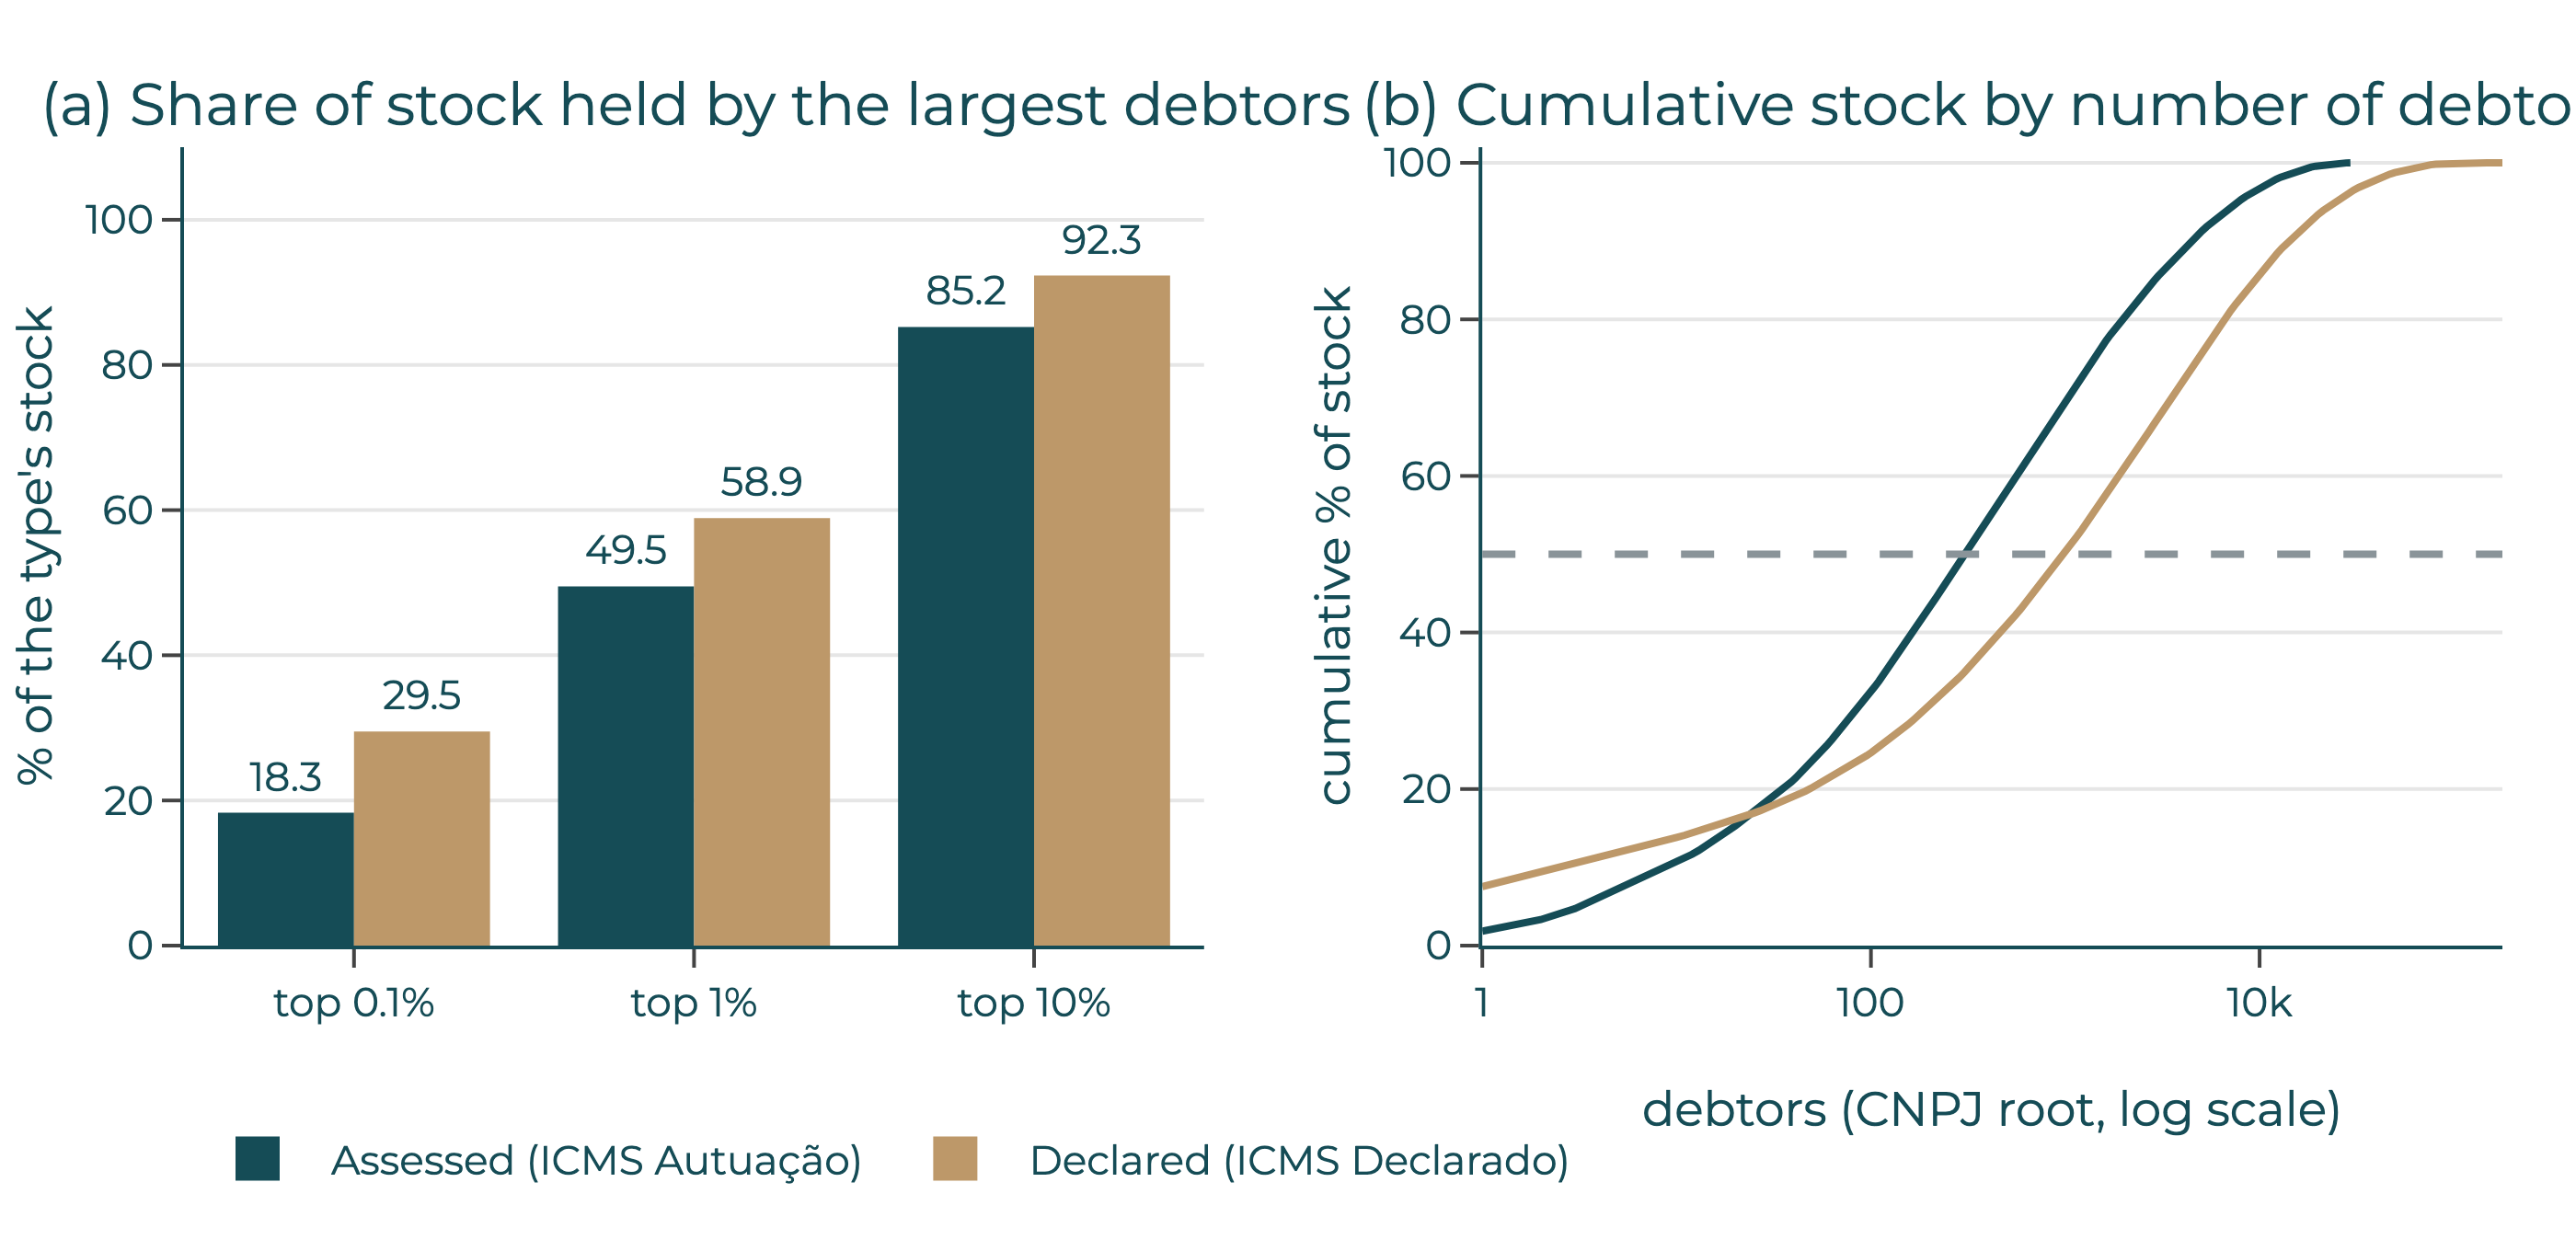
\includegraphics[width=\linewidth]{figures/fig_concentration_origin.png}
\caption{Share of each origin's stock held by the largest debtors (a) and cumulative stock by number of debtors, log scale (b). December 2025.}\label{fig:conc}
\end{figure}

\subsection{Recovery over time, and three open questions}\label{sec:res-series}
From 2016 to 2025, the annual recovery rate ranged from \rateMinDeclared\% (\rateMinYearDeclared) to \rateMaxDeclared\% (\rateMaxYearDeclared) for declared debt and from \rateMinAssessed\% (\rateMinYearAssessed) to \rateMaxAssessed\% (\rateMaxYearAssessed) for assessed debt (Figure~\ref{fig:series}).
In 2025 the rates were \rateTwentyFiveDeclared\% and \rateTwentyFiveAssessed\%.

The assessed series has three features this paper does not explain, registered as open research questions:
\begin{itemize}
\item \textbf{RQ-A, the 2020 fall.} The number of assessed CDAs in the panel falls from \cdaAssessedNineteen{} in 2019 to \cdaAssessedTwenty{} in 2020. Is it an artefact of the missing October--December 2020 snapshots, or a change in the assessed portfolio?
\item \textbf{RQ-B, the 2019 and 2024 peaks.} Assessed payments reach BRL~\paidAssessedNineteen{} billion in 2019 and BRL~\paidAssessedTwentyFour{} billion in 2024. Are the peaks related to instalment programmes or settlement agreements in those years, or to a few very large payments? Answering requires payment-level timing and the programme rules.
\item \textbf{RQ-C, data.} Do the comparisons by origin hold when the panel is re-run on a \texttt{DEBITO} table without missing and partial snapshots?
\end{itemize}
No cause is asserted for any of them; the series will be re-run once the missing snapshots are restored.

\begin{figure}[H]\centering
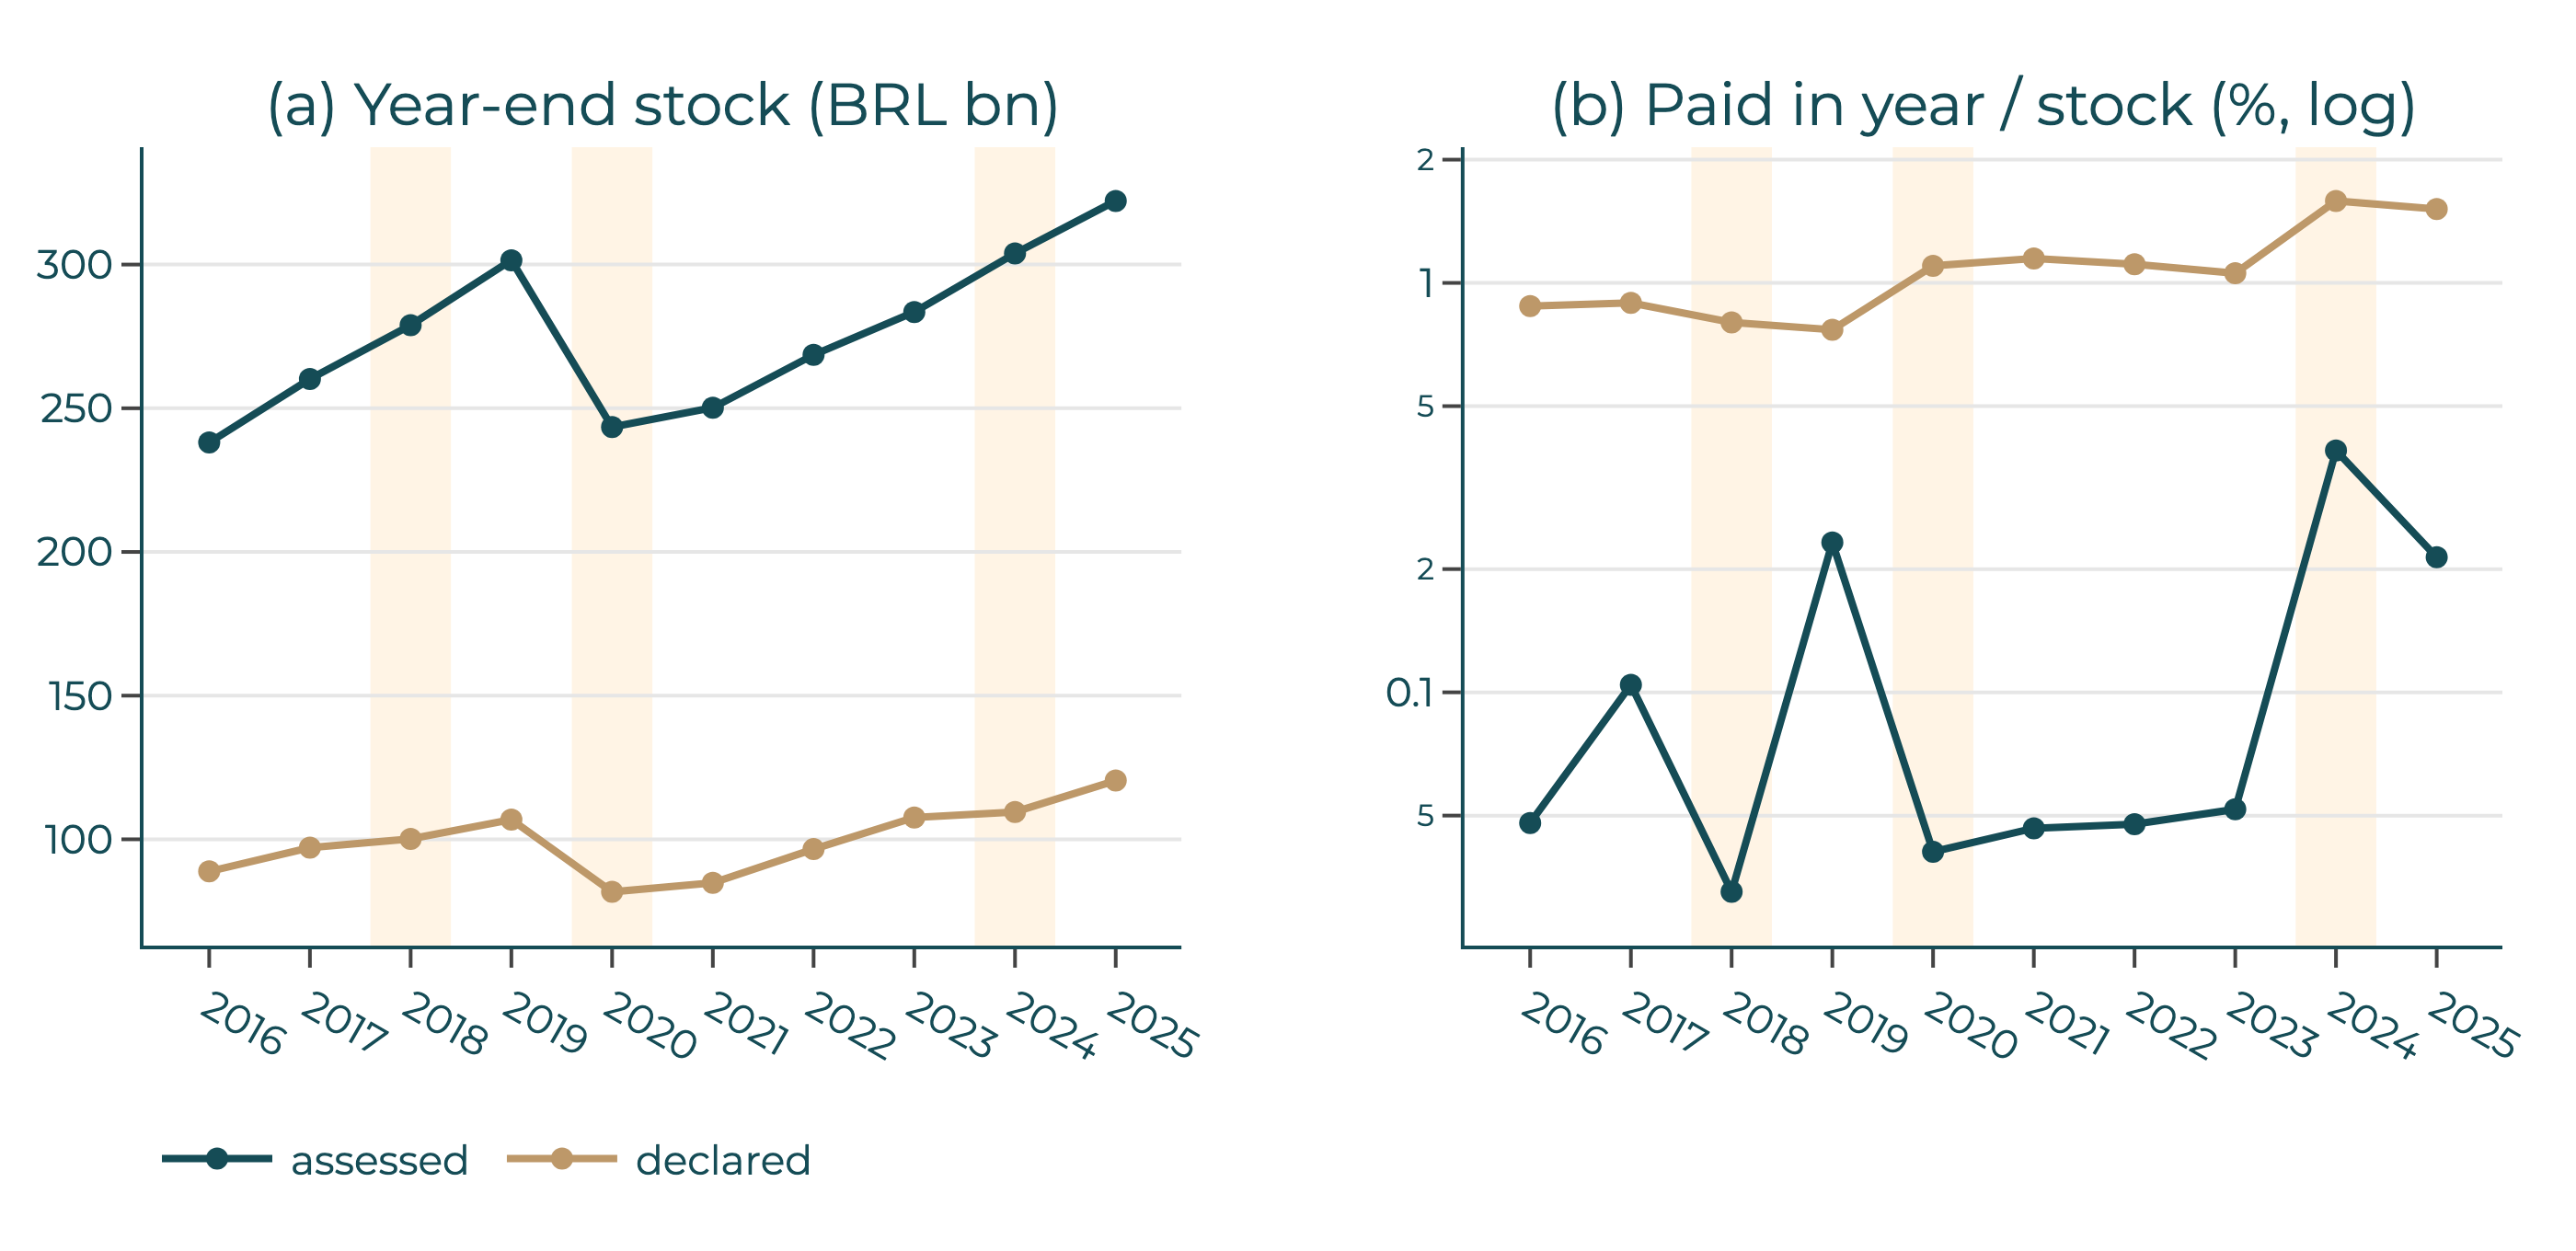
\includegraphics[width=\linewidth]{figures/fig_annual_series_origin.png}
\caption{Year-end stock (a) and annual recovery rate, log scale (b), by origin, legal entities, 2016--2025. Shaded years have missing (2018, 2020) or partial (2024) snapshots.}\label{fig:series}
\end{figure}

\subsection{The largest debts}\label{sec:res-top}
Among the largest 1\% of legal-entity CDAs (\kmN{} CDAs, at least BRL~\kmMinValueMn{} million each, BRL~\kmSumBn{} billion in total), \topOnePctCdaAssessed\% are assessed and they carry \topOnePctValueAssessed\% of the value.
In the rest of the portfolio (outside the top 1\%), \restOnePctCdaAssessed\% of the CDAs are assessed, with \restOnePctValueAssessed\% of the value (Table~\ref{tab:top}).
In the finer cut of the top 0.1\%, \topTenthPctCdaAssessed\% of the CDAs are assessed.

\begin{table}[H]\centering\small
\caption{Assessed share among the largest legal-entity CDAs, December 2025. The rest is everything outside the top 1\%.}\label{tab:top}
% generated by projects/macro/notebooks/articles/icms_declarado_autuado.ipynb; do not edit by hand
% Assessed share among the largest legal-entity CDAs, December 2025; rest = outside the top 1%
\begin{tabular}{lrrr}
\toprule
set of CDAs & assessed CDAs & assessed share of CDAs (\%) & assessed share of value (\%) \\
\midrule
top 0.1\% & 2,180 & 93.9 & 93.5 \\
top 1\% & 18,283 & 78.7 & 90.7 \\
rest (outside top 1\%) & 41,011 & 1.8 & 16.6 \\
\bottomrule
\end{tabular}

\end{table}

Inside the top 1\%, the silhouette at $k=4$ is \kmSilEuclid{} (Euclidean) and \kmSilGower{} (Gower).
The four groups split mainly by origin (Table~\ref{tab:km}); the largest, G1, has \kmGOnePctCda\% of the CDAs and \kmGOnePctValue\% of the value.
Origin is one of the clustering inputs, so this separation is partly built in.
Without origin, the adjusted Rand index between the two partitions is \kmNoOriginAri{} (1 = same partition, 0 = chance agreement) and the origin purity of the clusters falls from \kmPurityWith\% to \kmPurityWithout\%, the level of the largest origin in the top 1\% (\kmPurityBase\%).
\discutir{whether origin should be read as the axis that separates the largest debts}

\begin{table}[H]\centering\small
\caption{K-means ($k=4$) on the top 1\% of legal-entity CDAs, December 2025. Modal labels are translated from the raw database values.}\label{tab:km}
\resizebox{\linewidth}{!}{% generated by projects/macro/notebooks/articles/icms_declarado_autuado.ipynb; do not edit by hand
% K-means (k = 4) on the top 1% of legal-entity CDAs, December 2025; modal labels translated from the raw database values
\begin{tabular}{lrrrrrrrr}
\toprule
cluster & CDAs (\%) & value (\%) & modal origin & modal situation & modal filing status & median value (BRL mn) & median age (years) & any payment (\%) \\
\midrule
G1 & 70.7 & 79.7 & assessed (100.0\%) & enrolled & filed in court & 4.69 & 10.0 & 12.5 \\
G2 & 19.6 & 8.8 & declared (100.0\%) & enrolled & filed in court & 2.47 & 9.6 & 12.0 \\
G3 & 6.4 & 6.1 & assessed (77.2\%) & enrolled & cleared for filing & 3.83 & 0.8 & 16.5 \\
G4 & 3.3 & 5.4 & assessed (94.0\%) & suspended & filed in court & 5.27 & 6.1 & 6.1 \\
\bottomrule
\end{tabular}
}
\end{table}

\subsection{Debtor firm characteristics (descriptors only)}\label{sec:res-firms}
Registration status and economic activity are measured in March 2026, after the outcomes, and describe the debtors of each origin; they are not causes.

\paragraph{Registration status.}
Firms active in March 2026 hold \stPctStockAssessedActive\% of the assessed and \stPctStockDeclaredActive\% of the declared stock; firms declared unfit (\emph{inapta}) hold \stPctStockAssessedUnfit\% and \stPctStockDeclaredUnfit\% (Table~\ref{tab:status}).
The pooled 2016--2025 recovery rate of assessed debt is \stRecoveryAssessedActive\% for active firms and \stRecoveryAssessedUnfit\% for unfit firms; for declared debt it is \stRecoveryDeclaredActive\% and \stRecoveryDeclaredUnfit\%.
In the 2016--2025 enrolment cohort, \kmPaidFiveYrAssessedActive\% of assessed CDAs of active firms had a first payment within 60 months, against \kmPaidFiveYrAssessedUnfit\% for unfit firms (Figure~\ref{fig:km}).
A firm may be closed or unfit \emph{because} of its debts, so these differences are associations.

\begin{table}[H]\centering\small
\caption{Registration status of the debtor CNPJ (RFB, March 2026) by origin. Descriptors only. KM: Kaplan--Meier share of CDAs of the 2016--2025 enrolment cohort with a first payment by 12 and 60 months; empty cells have no CDA in the cohort.}\label{tab:status}
\resizebox{\linewidth}{!}{% generated by projects/macro/notebooks/articles/icms_declarado_autuado.ipynb; do not edit by hand
% Registration status of the debtor CNPJ (RFB, March 2026) by origin, descriptors only; KM = Kaplan-Meier share with a first payment, enrolment cohort 2016-2025
\begin{tabular}{lrrrrrrr}
\toprule
origin & status (Mar 2026) & CNPJs & share of origin stock (\%) & any payment (\%) & pooled recovery (\%) & KM 12 m (\%) & KM 60 m (\%) \\
\midrule
assessed & active & 15,640 & 52.9 & 30.8 & 0.22 & 18.9 & 35.1 \\
assessed & unfit (inapta) & 9,243 & 21.7 & 5.5 & 0.01 & 2.9 & 6.8 \\
assessed & suspended & 275 & 1.2 & 14.0 & 0.02 & 8.1 & 22.3 \\
assessed & closed (baixada) & 7,625 & 24.1 & 8.0 & 0.10 & 11.4 & 22.6 \\
assessed & null (nula) & 25 & 0.0 & 5.6 & 0.00 & 2.1 & 2.1 \\
assessed & root only (status unknown) & 193 & 0.0 & 0.7 & 0.00 &  &  \\
assessed & not found in register & 138 & 0.0 & 0.7 & 0.01 &  &  \\
declared & active & 142,869 & 74.4 & 30.4 & 1.70 & 30.2 & 36.5 \\
declared & unfit (inapta) & 20,994 & 15.2 & 7.0 & 0.07 & 8.6 & 10.3 \\
declared & suspended & 806 & 0.5 & 13.9 & 0.52 & 13.1 & 16.5 \\
declared & closed (baixada) & 29,882 & 9.7 & 16.9 & 0.47 & 22.7 & 27.5 \\
declared & null (nula) & 80 & 0.1 & 10.3 & 0.11 & 10.3 & 12.5 \\
declared & root only (status unknown) & 140 & 0.1 & 1.2 & 0.01 &  &  \\
declared & not found in register & 72 & 0.0 & 0.3 & 0.00 &  &  \\
\bottomrule
\end{tabular}
}
\end{table}

\begin{figure}[H]\centering
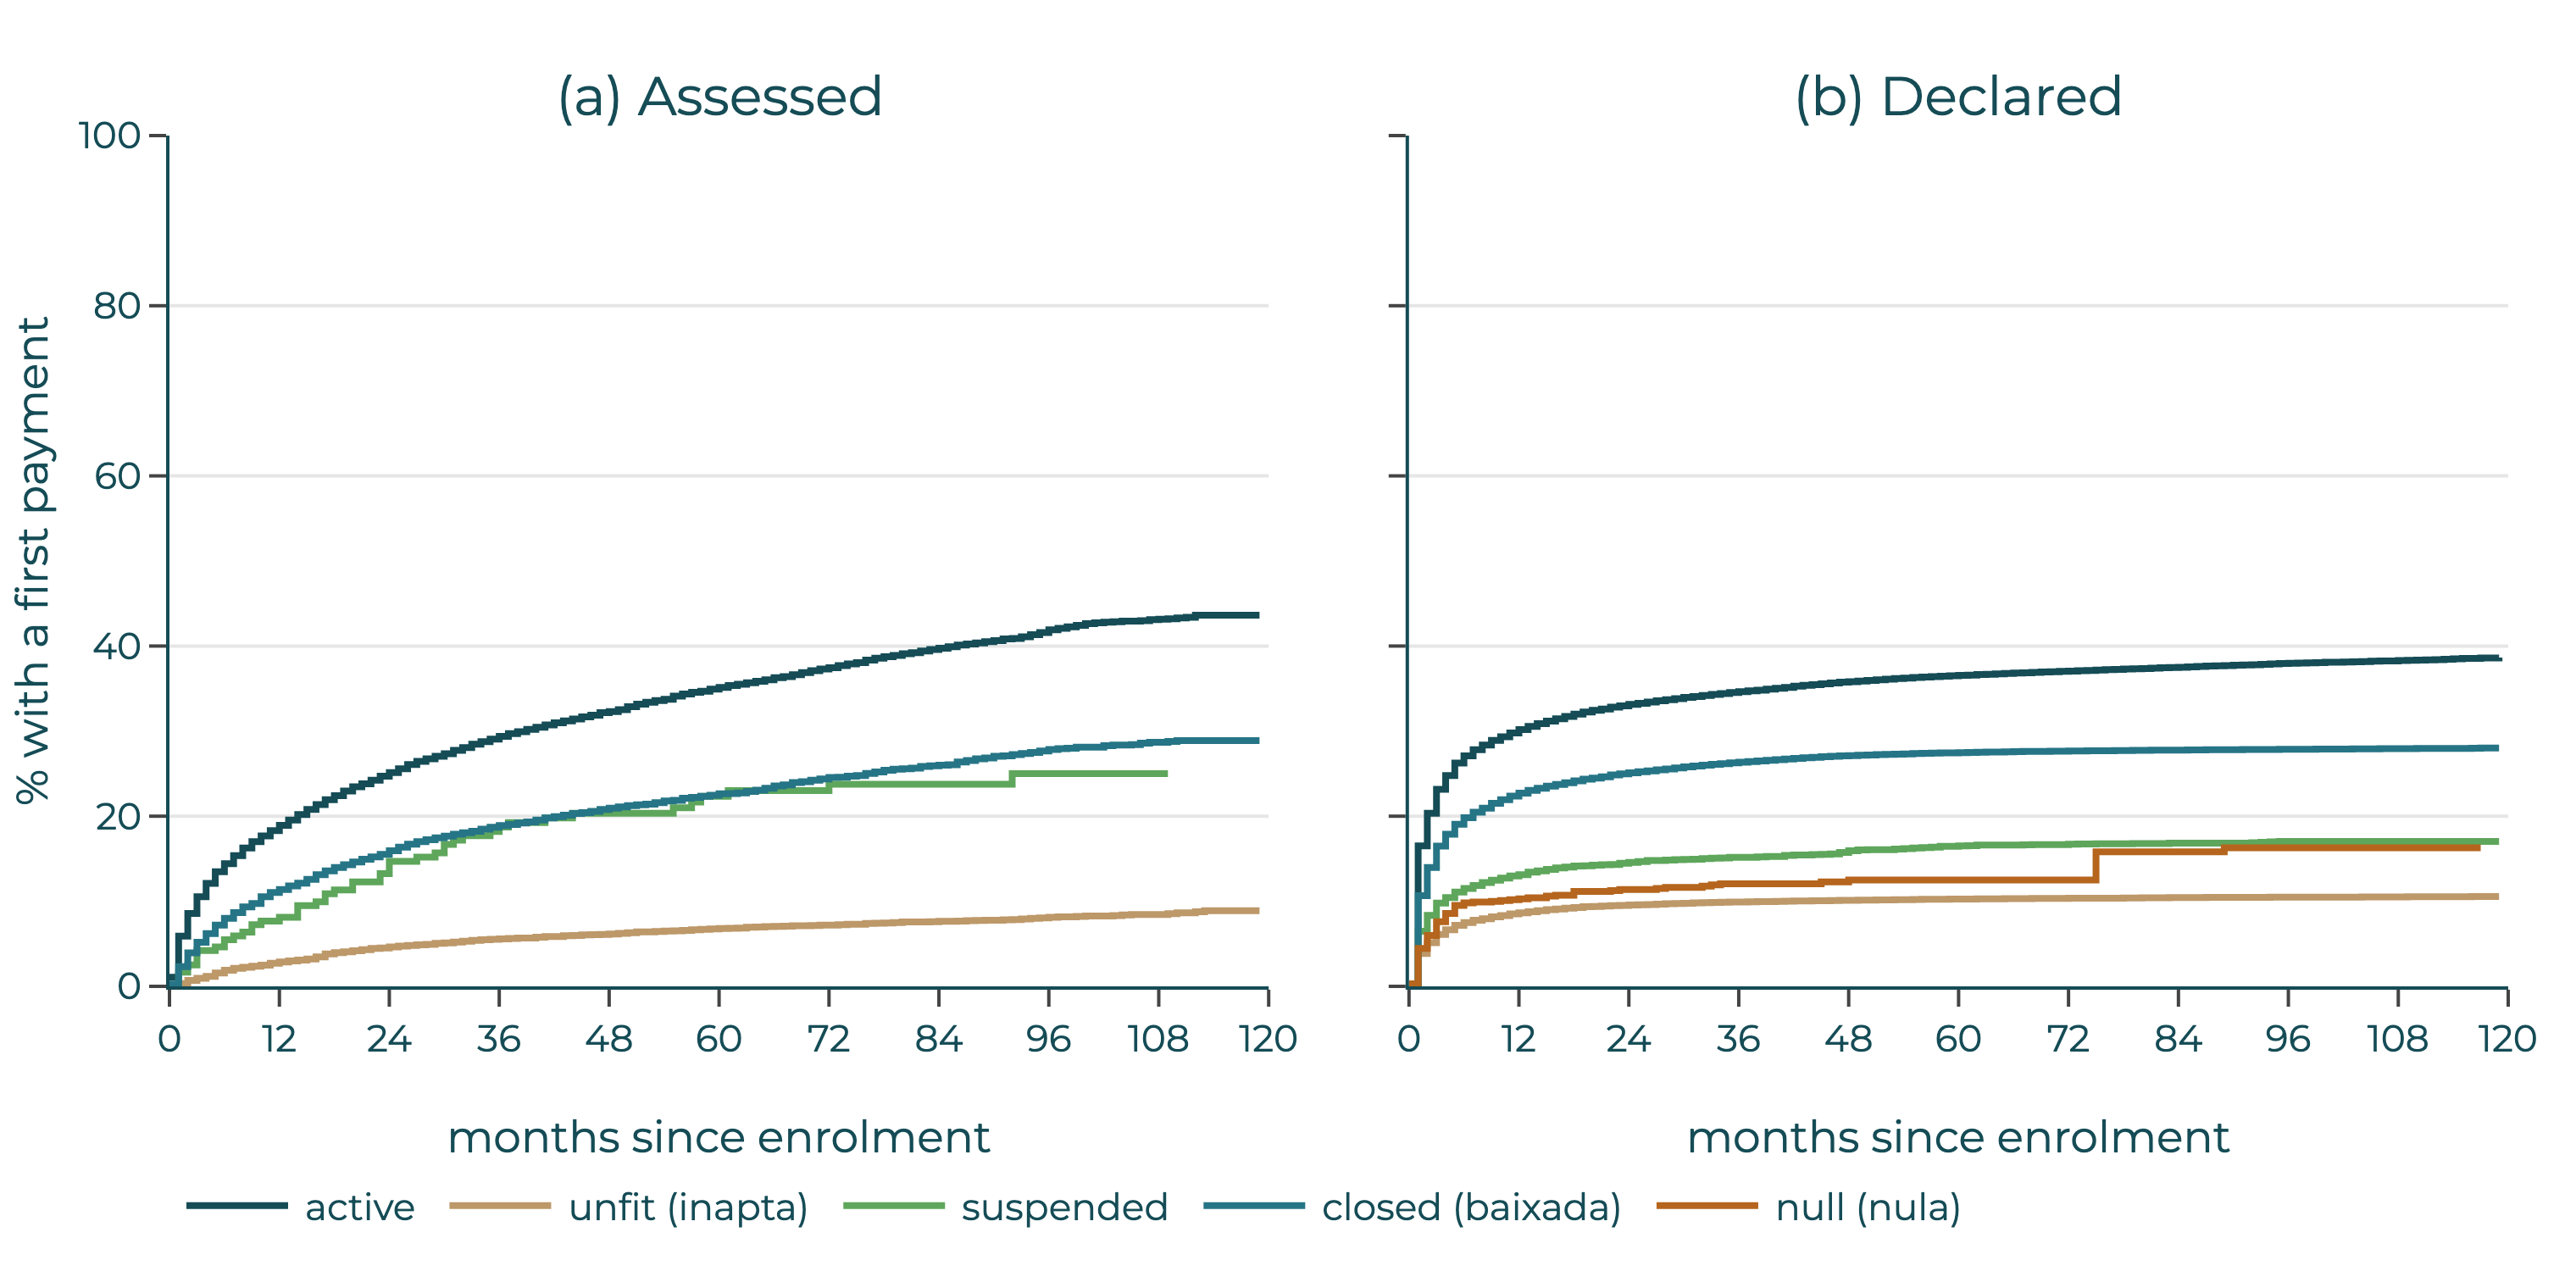
\includegraphics[width=\linewidth]{figures/fig_km_status_origin.png}
\caption{Kaplan--Meier share of CDAs with a first payment by months since enrolment, by registration status: assessed (a) and declared (b). Enrolment cohort 2016--2025.}\label{fig:km}
\end{figure}

\paragraph{Economic activity.}
The ten largest CNAE divisions hold \cnaeTenPctStock\% of the December 2025 \vat{} stock (Table~\ref{tab:cnae}).
The largest is division \cnaeTopDivision{} (\cnaeTopDivisionName), with \cnaeTopDivisionPctStock\% of the stock, \cnaeTopDivisionAssessedWeight\% of it assessed; the second is division \cnaeSecondDivision{} (\cnaeSecondDivisionName), with \cnaeSecondDivisionPctStock\%, \cnaeSecondDivisionAssessedWeight\% assessed.
Across the \cnaeNDivShown{} divisions shown, the assessed share of the stock ranges from \cnaeAssessedWeightMin\% to \cnaeAssessedWeightMax\%, and its Spearman correlation with the division's pooled recovery rate is \cnaeSpearman{} (Figure~\ref{fig:cnae}); this is an ecological description, not a within-division comparison.
\cnaeNDivSuppressed{} divisions are pooled for disclosure control.
\discutir{which divisions, if any, the text names and comments on}

\begin{table}[H]\centering\small
\caption{Ten largest CNAE 2.0 divisions by December 2025 \vat{} stock. Assessed weight: assessed share of the division's stock. Recovery: pooled 2016--2025 rate by origin. English names translated from the official Portuguese names. Descriptors only.}\label{tab:cnae}
\resizebox{\linewidth}{!}{% generated by projects/macro/notebooks/articles/icms_declarado_autuado.ipynb; do not edit by hand
% Ten largest CNAE divisions by December 2025 VAT (ICMS) stock: assessed weight and pooled 2016-2025 recovery by origin; descriptors only
\begin{tabular}{lrrrrr}
\toprule
division & activity (CNAE 2.0, English) & share of VAT stock (\%) & assessed weight (\%) & recovery, assessed (\%) & recovery, declared (\%) \\
\midrule
46 & Wholesale trade, except motor vehicles and motorcycles & 27.3 & 85.6 & 0.09 & 0.95 \\
47 & Retail trade & 11.8 & 72.5 & 0.13 & 1.44 \\
10 & Manufacture of food products & 6.6 & 82.4 & 0.12 & 1.56 \\
49 & Land transport & 5.6 & 43.1 & 0.28 & 1.19 \\
61 & Telecommunications & 4.2 & 96.5 & 0.33 & 1.85 \\
24 & Metallurgy & 4.0 & 86.5 & 0.06 & 0.86 \\
19 & Manufacture of coke, petroleum products and biofuels & 3.7 & 28.3 & 0.11 & 0.30 \\
82 & Office and administrative support services and other services mainly to businesses & 3.7 & 77.8 & 0.10 & 1.16 \\
22 & Manufacture of rubber and plastic products & 3.4 & 59.9 & 0.16 & 0.98 \\
25 & Manufacture of metal products, except machinery and equipment & 3.1 & 53.3 & 0.11 & 0.93 \\
\bottomrule
\end{tabular}
}
\end{table}

\begin{figure}[H]\centering
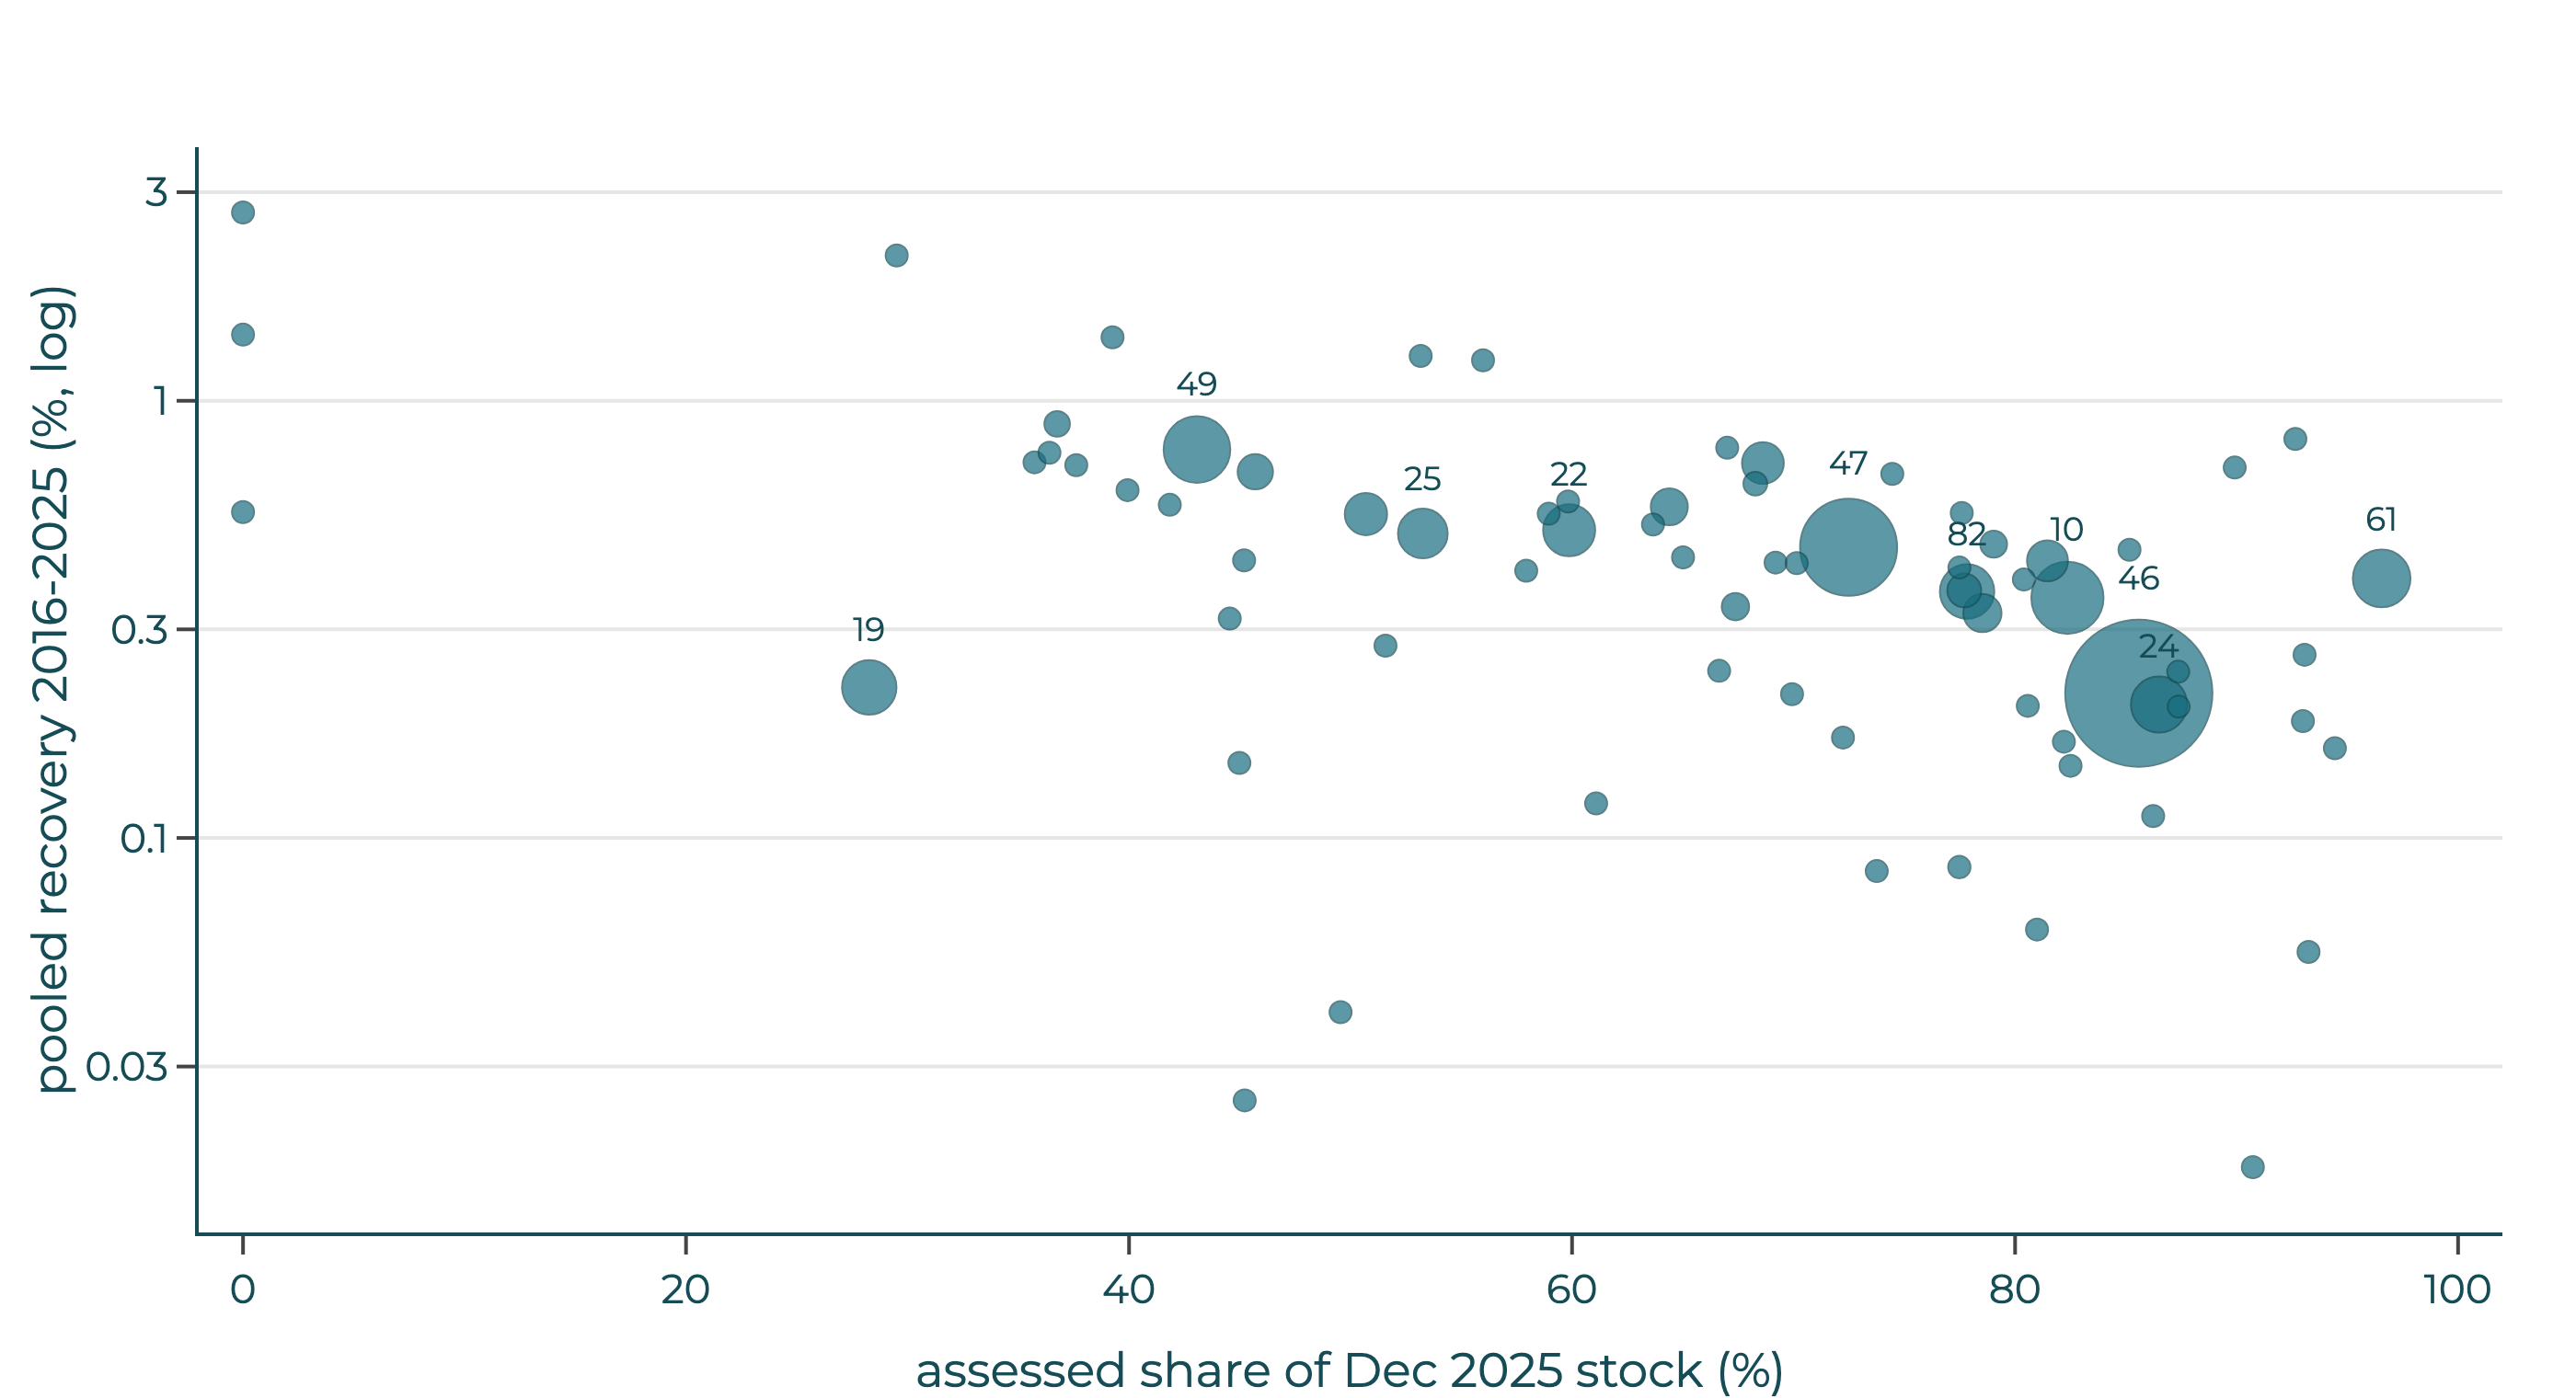
\includegraphics[width=0.85\linewidth]{figures/fig_cnae_division_origin.png}
\caption{CNAE divisions: assessed share of the December 2025 stock (horizontal) and pooled 2016--2025 recovery rate, log scale (vertical). Bubble area is proportional to the division's stock; the ten largest are labelled with their code.}\label{fig:cnae}
\end{figure}

\section{Discussion}\label{sec:discussion}
\discutir{interpretation of the results: what separating declared and assessed debt means for VAT compliance studies and for debt collection; links to \citet{keen2006}, \citet{kleven2011} and \citet{pomeranz2015}}

\discutir{scope of the Brazil--Italy comparison with Prof.\ L\'ivia, if it stays in this paper}

\section{Open questions and limitations}\label{sec:limits}
\begin{itemize}
\item \textbf{Data gaps.} Missing and partial \texttt{DEBITO} snapshots (Section~\ref{sec:data}, Appendix~\ref{app:quality}) affect the annual series; RQ-A to RQ-C (Section~\ref{sec:res-series}) remain open, with no cause asserted.
\item \textbf{Definition of declared debt.} The legal meaning of \texttt{ICMS Declarado} is to be confirmed with PGE-SP.
\item \textbf{Independence.} Rank tests assume independent CDAs, which fails when one debtor has several CDAs; debtor-level tests or resampling by debtor are the next step.
\item \textbf{Clustering.} Origin is a clustering input; the without-origin sensitivity limits any claim that origin separates the largest debts.
\item \textbf{Firm register.} Registration status and CNAE come from the Receita Federal CNPJ registry and are observed after the outcomes. They are descriptors, not causes. Censoring in the Kaplan--Meier curves is assumed independent of payment within each group, a strong assumption for closed or unfit firms.
\item \textbf{Programme windows.} The instalment-programme windows used as a clustering input are inherited from earlier work and must be confirmed.
\end{itemize}

\section{Conclusion}\label{sec:conclusion}
\discutir{conclusions of the authors}

\paragraph{Data and code.}
All numbers, tables and figures are generated by one notebook (\texttt{projects/macro/notebooks/articles/icms\_declarado\_autuado.ipynb}) that reads the pinned database in read-only mode and publishes aggregates only; cells with fewer than five distinct firms are pooled.
The underlying records are confidential tax data of PGE-SP and cannot be shared.

\paragraph{Use of AI.}
An AI assistant helped assemble the notebook and this draft; the analysis choices, the interpretation and the conclusions are the authors'. \discutir{wording of the AI statement}


\bibliographystyle{plainnat}
\bibliography{refs}

\appendix
\section{Quality of the monthly snapshots}\label{app:quality}
Missing snapshots: \qualMissingSnapshots.
Possibly partial snapshots (fewer than 80\% of the CDAs of the centred 7-snapshot rolling median): \qualPartialSnapshots.
Snapshots with duplicated rows (counted once): \qualDuplicatedSnapshots.

\begin{figure}[H]\centering
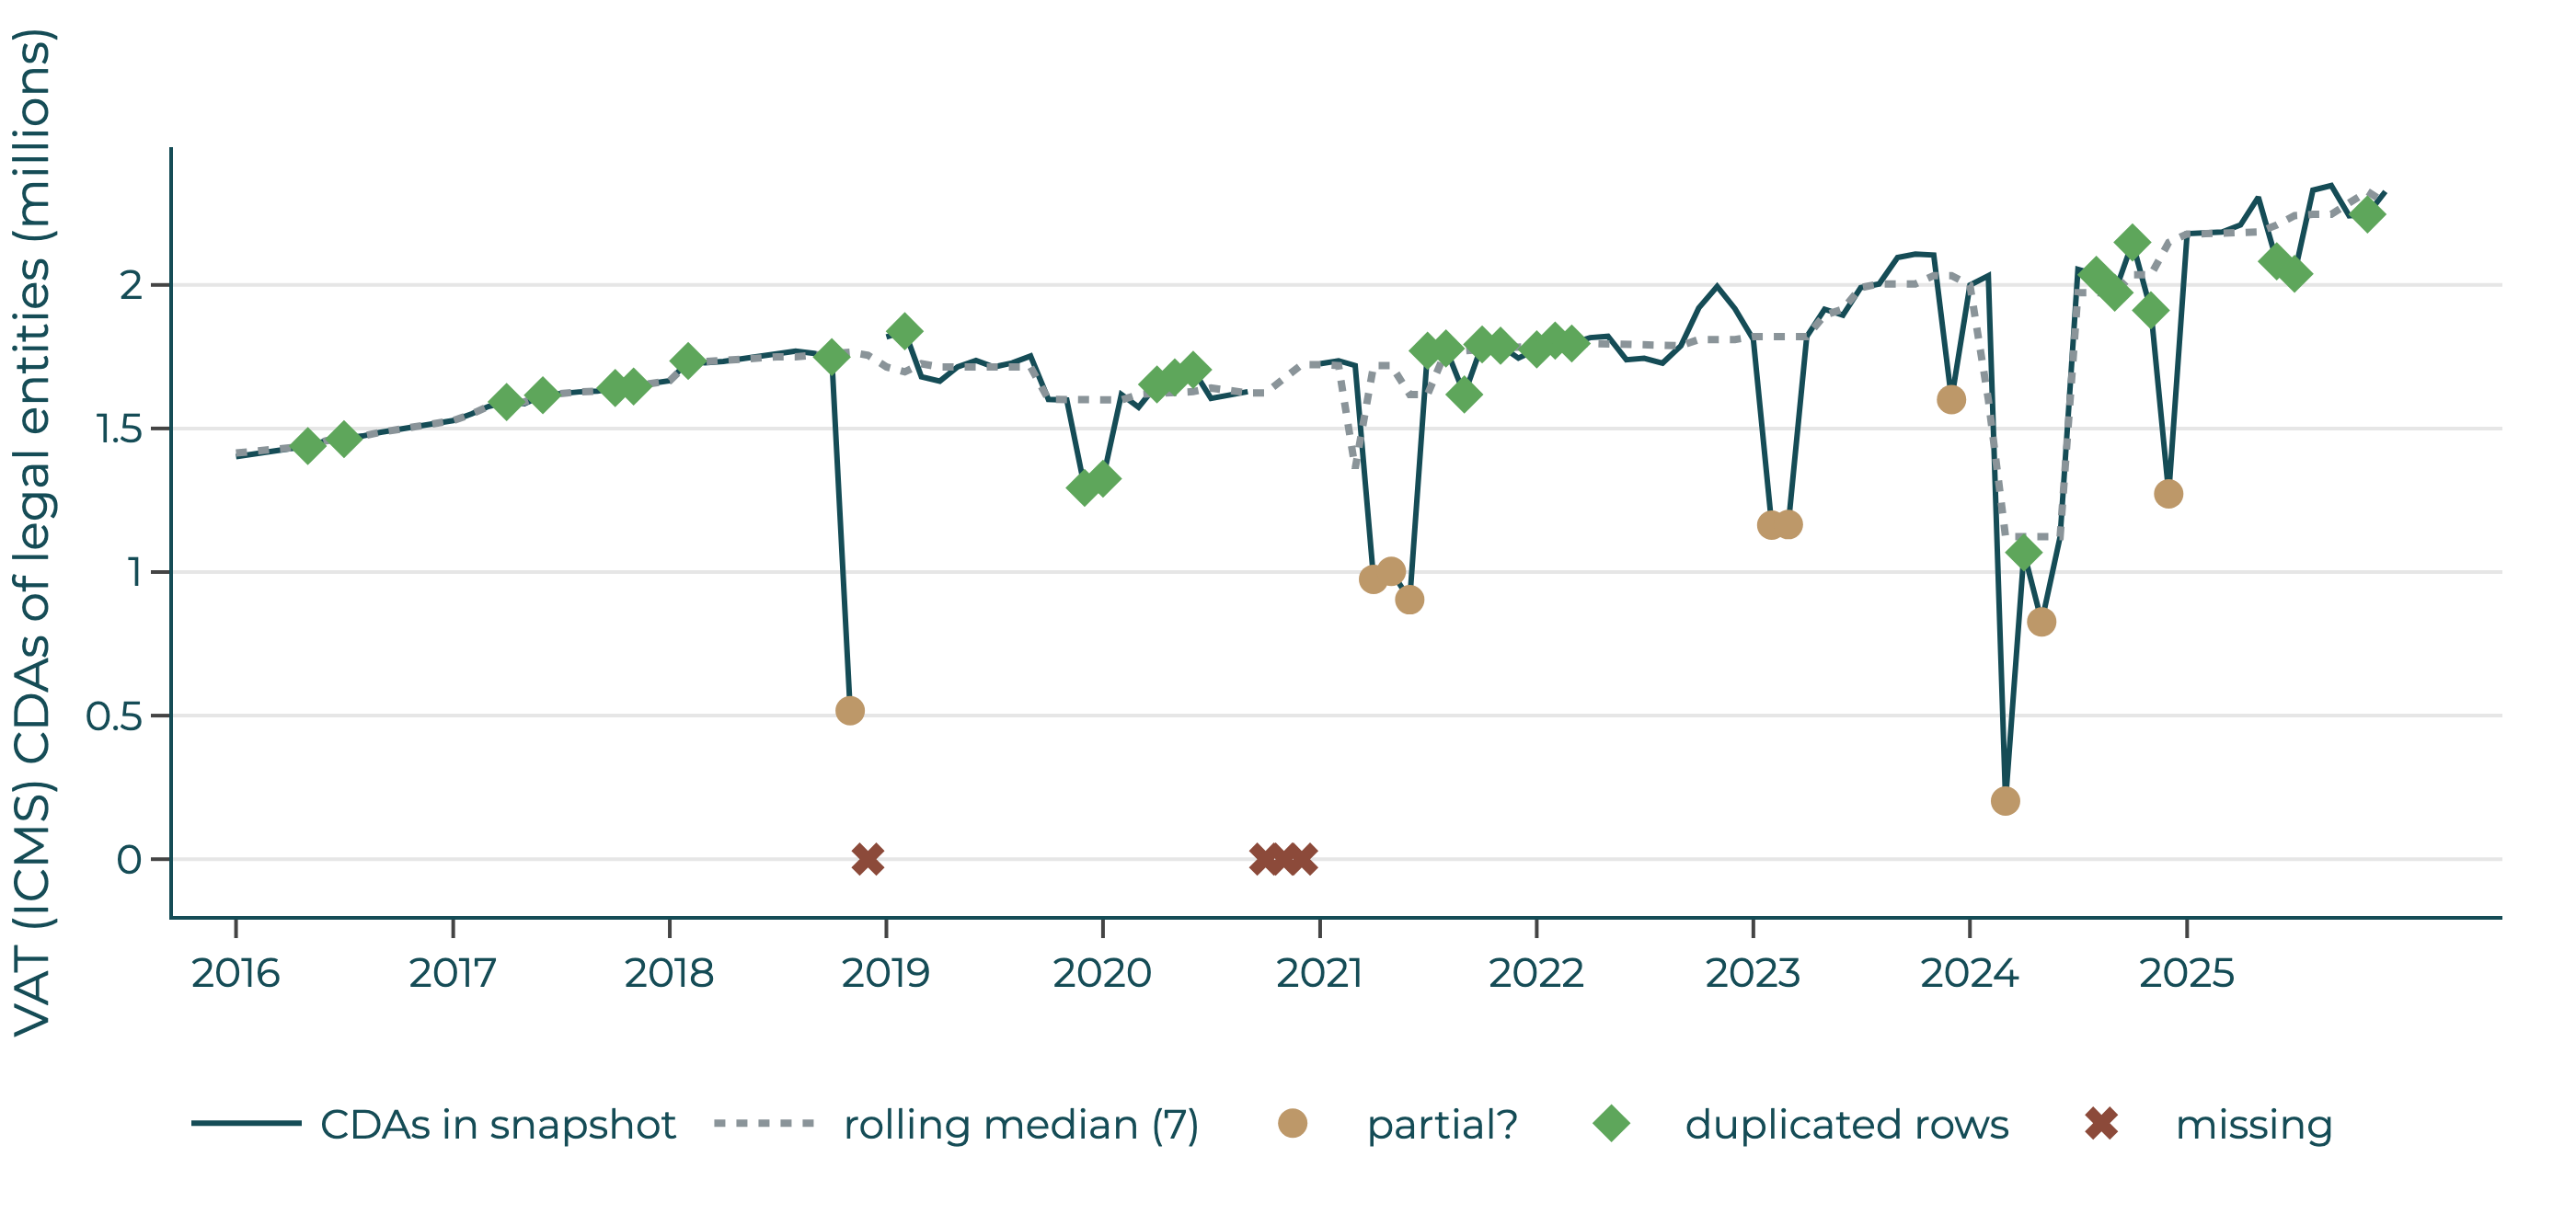
\includegraphics[width=\linewidth]{figures/fig_debito_quality.png}
\caption{Distinct \vat{} CDAs of legal entities in each monthly snapshot, 2016--2025, with the rolling reference and flagged snapshots.}\label{fig:quality}
\end{figure}

\section{Additional tables}\label{app:tables}

\begin{table}[H]\centering\small
\caption{K-means on the top 1\%: silhouette by $k$ (5,000-CDA subsample; 100 initialisations per $k$).}
% generated by projects/macro/notebooks/articles/icms_declarado_autuado.ipynb; do not edit by hand
% K-means on the top 1%: silhouette by k (5,000 subsample), 100 initialisations per k
\begin{tabular}{lrrrr}
\toprule
k & inertia & silhouette\_euclid & silhouette\_gower & smallest\_cluster\_pct \\
\midrule
2 & 4,420.7 & 0.602 & 0.600 & 21.3 \\
3 & 2,870.1 & 0.658 & 0.648 & 8.0 \\
4 & 2,380.7 & 0.676 & 0.661 & 3.3 \\
5 & 2,075.4 & 0.593 & 0.596 & 3.3 \\
6 & 1,794.0 & 0.608 & 0.606 & 1.7 \\
7 & 1,531.1 & 0.450 & 0.421 & 1.7 \\
8 & 1,320.8 & 0.464 & 0.431 & 1.5 \\
\bottomrule
\end{tabular}

\end{table}

\begin{table}[H]\centering\small
\caption{Coverage of the join with the RFB register (March 2026), legal-entity \vat{} CDAs, by origin.}
\resizebox{\linewidth}{!}{% generated by projects/macro/notebooks/articles/icms_declarado_autuado.ipynb; do not edit by hand
% Coverage of the join with the Receita Federal CNPJ registry (cnpj_enriquecido), legal-entity VAT (ICMS) CDAs, by origin
\begin{tabular}{lrrrrrrrr}
\toprule
origin & match\_level & cdas\_dec2025 & stock\_dec2025\_bn & cnpjs\_dec2025 & cdas\_panel & pct\_cdas\_dec2025 & pct\_stock\_dec2025\_bn & pct\_cdas\_panel \\
\midrule
assessed & estabelecimento & 58,903 & 311.2 & 32,808 & 156,873 & 99.3 & 99.9 & 98.1 \\
assessed & nao\_encontrado & 175 & 0.1 & 138 & 901 & 0.3 & 0.0 & 0.6 \\
assessed & raiz & 216 & 0.1 & 193 & 2,216 & 0.4 & 0.0 & 1.4 \\
declared & estabelecimento & 2,253,855 & 116.3 & 194,631 & 4,771,940 & 100.0 & 99.9 & 99.9 \\
declared & nao\_encontrado & 90 & 0.0 & 72 & 595 & 0.0 & 0.0 & 0.0 \\
declared & raiz & 442 & 0.1 & 140 & 1,797 & 0.0 & 0.1 & 0.0 \\
\bottomrule
\end{tabular}
}
\end{table}

\begin{figure}[H]\centering
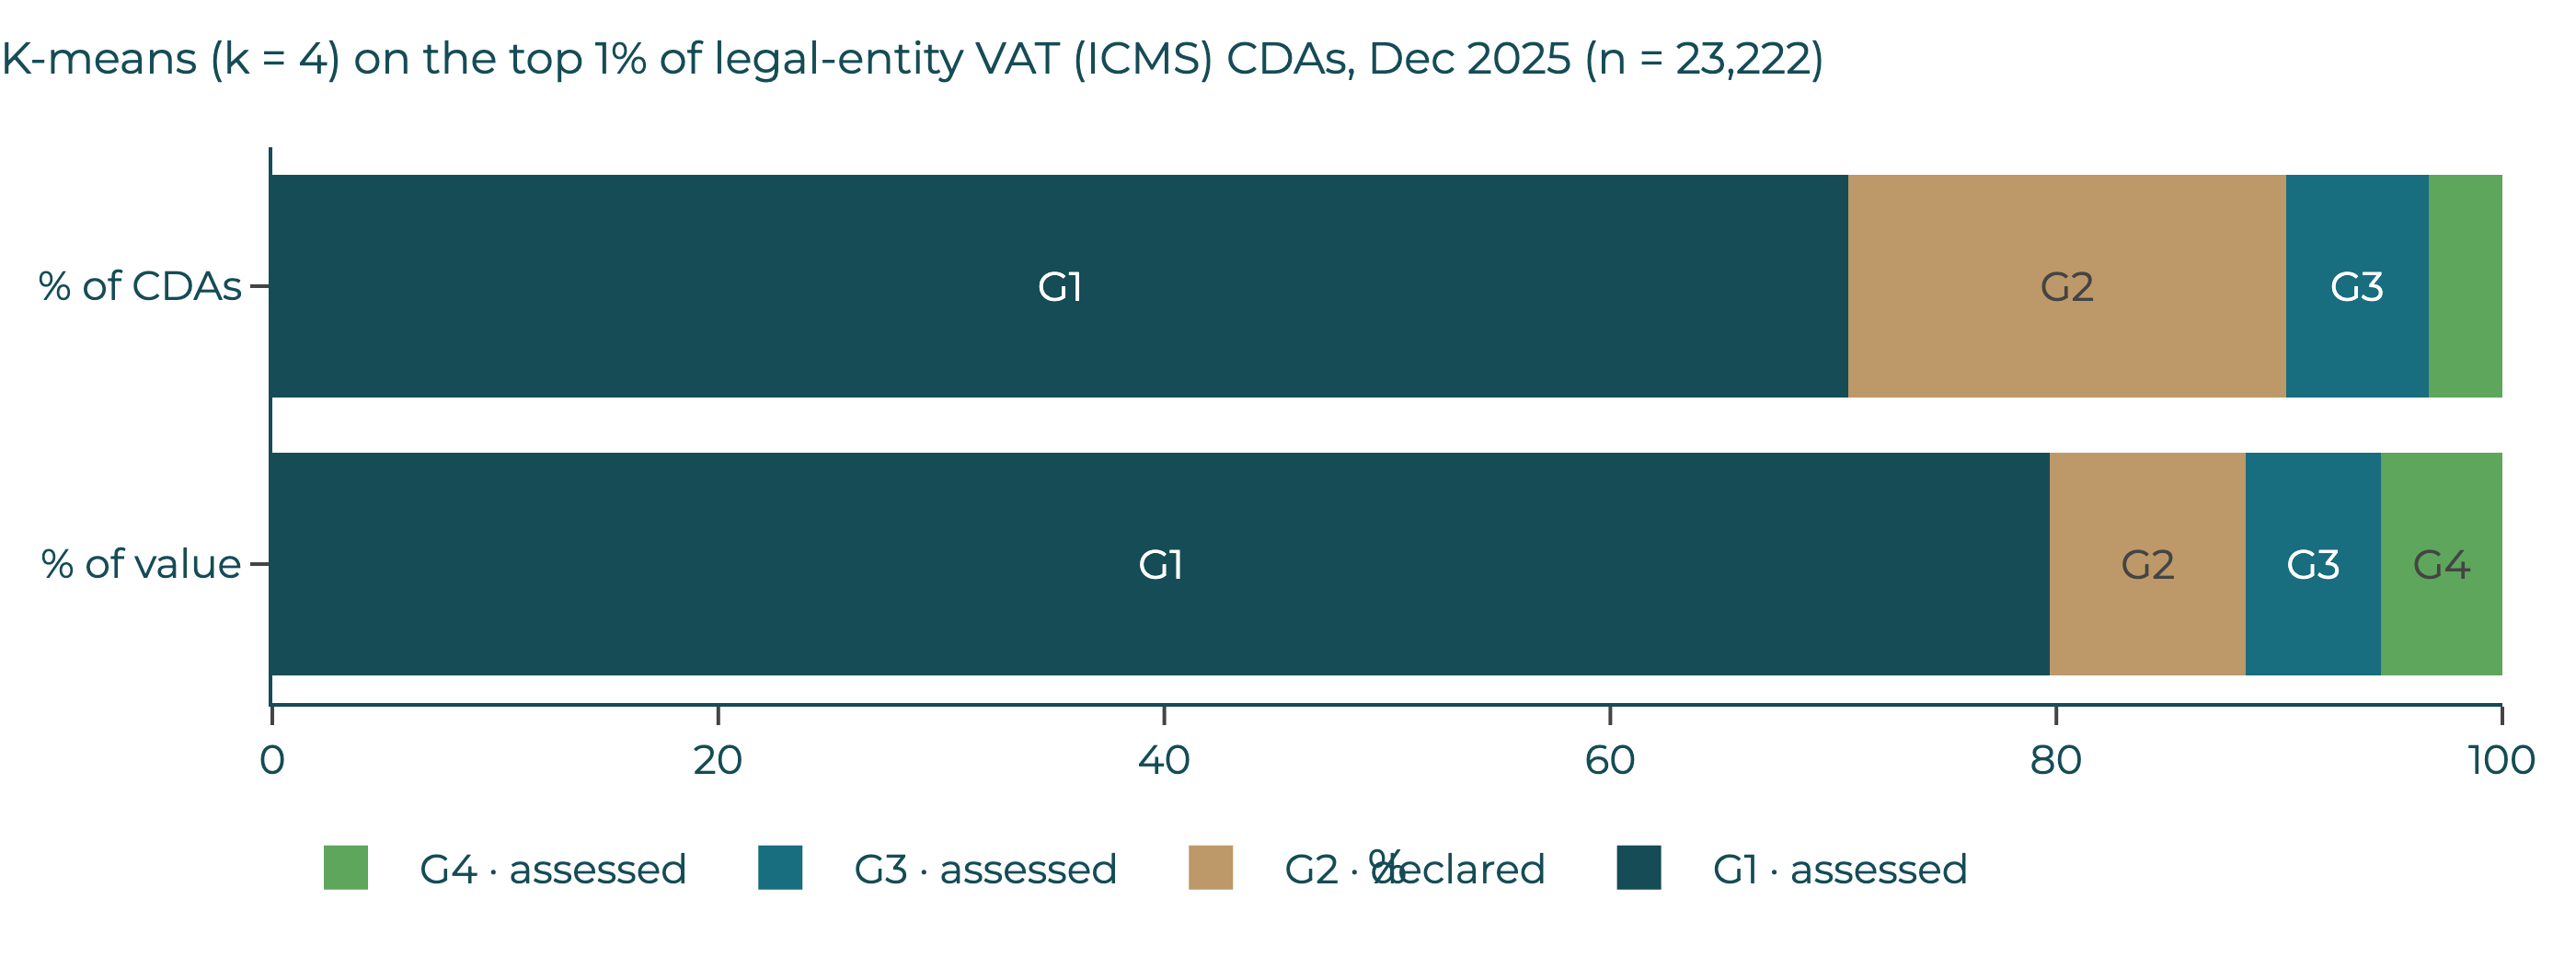
\includegraphics[width=\linewidth]{figures/fig_kmeans_k4_top1.png}
\caption{Composition of the four K-means clusters in the top 1\% of CDAs, by number and by value.}\label{fig:kmfig}
\end{figure}


\end{document}
